\documentclass{article}
\usepackage[francais]{babel}
\usepackage[utf8]{inputenc}
\usepackage{xcolor}
\usepackage[pdftex]{graphicx}
\usepackage{listings}
\usepackage{amsmath}
\usepackage[a4paper,includeheadfoot,margin=2.54cm]{geometry}
\usepackage{amsfonts}
\usepackage{fancyhdr}
\usepackage{titling}
\usepackage{algorithm}
\usepackage{algpseudocode}
\usepackage{hyperref}

\pagestyle{fancy}
\fancyhf{}
\fancyhead[LE,RO]{\theauthor}
\fancyhead[RE,LO]{\thetitle}
\fancyfoot[CE,CO]{\leftmark}
\fancyfoot[LE,RO]{\thepage}

\usepackage[thinlines]{easytable}

\title{Atelier d'approfondissement en informatique: Graphes et Algorithmes}
\author{Quentin Garrido}
\date{21 avril 2019}

\begin{document}

\maketitle
\tableofcontents
\pagebreak

%=============================================================================%
\section{Introduction}
\subsection{Objectifs}

L'objectif de ce projet est d'implémenter des algorithmes de recherche de plus courts
chemins dans un graphe, et plus particulièrement dans un graphe représentant le réseau
de métro de Paris.\\
Nous implémenterons tout d'abord l'algorithme de Dijkstra, puis le modifierons pour
qu'ils deviennent l'algorithme A* et nous optimiserons son temps d'éxécution grâce
à des structures de données adaptées.

\subsection{Utilisation}

Tout le code source est disponible à l'adresse suivante: \textit{https://github.com/garridoq/metro-shortest-path}.\\

Tout les éxécutables devraient vous être fournis dans le mail et devraient fonctionner sans devoir
les recompiler. Dans le cas contraire voici la démarche à suivre:\\

Un makefile est fourni pour la compilation, il servira à compiler les bibliothèques et les tests.
Une fois le code source obtenu il faudra exécuter la commande suivante pour compiler les bibliothèques:
\begin{lstlisting}[language=bash]
	> make
\end{lstlisting}

Vous pourrez alors compiler tous les fichiers de tests de la manière suivante:
\begin{lstlisting}[language=bash]
	> make NOM.exe
\end{lstlisting}
Où NOM est le nom du fichier de test (pour test\_heap.c, il faudra entrer make test\_heap.exe).\\

Voici la liste des fichiers de test et leur utilisation:
\begin{itemize}
	\item test\_heap:./test\_heap.exe , ce fichier permet de tester l'implémentation du tas
		  binaire et de ses opérations primaires.
	\item test\_dijkstra:./test\_dijkstra.exe GRAPH DEBUT FIN , ce fichier va récupérer
		  le graphe dans le fichier GRAPH, puis calculer le plus court chemin de DEBUT à FIN
		  en utilisant l'agorithme de Dijkstra, l'A* et A* avec une file de priorité.\\
		  Un fichier EPS sera créé pour chaque algorithme.\\
\end{itemize}

À titre de référence, voici à quoi ressemble le graphe entier du réseau de métro, que nous
utiliserons par la suite:
Les stations sont réprésentées par les sommets et nous avons une arc entre deux sommets
si ils sont reliés par le métro.

\begin{figure}[!hbt]
	\centering
	\includegraphics[width=\textwidth]{metro.eps}
	\caption{Graphe de référence du métro}
	\label{metro}
\end{figure}

\clearpage
%=============================================================================%
\section{Algorithme de Dijkstra}
\subsection{Implémentation}

Pour calculer le chemin de plus court d'un point D à A nous allons utiliser 
la version suivante de l'algorithme de Dijkstra, adaptée depuis le cours de 
l'unité Graphes et Algorithmes.\\

Ici nous n'avons pas besoin de calculer les chemins de notre sommet de départ
vers tous les autres sommets du graphe et nous nous arrêterons donc dès
que nous atteignons notre sommet d'arrivée.

\begin{algorithm}
\caption{Algorithme de Dijkstra}\label{dijkstra}
\begin{algorithmic}[1]
\Procedure{DIJKSTRA}{$E, \Gamma, l, d \in E, a \in E$}
	\State S = \{d\}, $\pi(d)$ = 0, k = 1, $x_1$ = d
	\ForAll{$x \in E$\textbackslash$ \{d\}$}
		\State $\pi(x) = \infty$
	\EndFor
	
	\While{$k < n$ et $\pi(x_k) < \infty$ }
		\ForAll{$y \in \Gamma(x_k) $ tel que $y \not\in S$}
			\State $\pi(y) = $ min[$\pi(y), \pi(x_k) + l(x_k, y)$]
		\EndFor
		\State Extraire $x \not\in S$ tel que $\pi(x)$=min$\{\pi(y), y \not\in S\}$
		\State k = k + 1, $x_k = x$, S = S $\bigcup \{x_k\}$
		\If{$x_k = a$}
			\State \textbf{break}
		\EndIf
	\EndWhile
	
	\State \textbf{return} $\pi$, S
\EndProcedure
\end{algorithmic}
\end{algorithm}

Nous implémentons S avec un tableau de $n = \vert E\vert$ éléments, correspondants aux sommets 
de notre graphe.\\
Ainsi nous l'initialiserons entièrement à 0 et S = S $\bigcup \{x_k\}$
correspondra à faire S[k] = 1.\\
Bien que cette implémentation soit plus coûteuse en mémoire qu'une liste chaînée
elle permettra d'implémenter l'appartenance à S en temps constant, opération très
utilisée aux lignes 7 et 10.\\
De plus l'ajout d'un élément sera aussi simplifié car nous n'aurons pas à vérifier
l'appartenance avant de l'insérer ou non.\\

\subsection{Récupération du plus court chemin}


Soit $c$ notre chemin de coût minimum, pour tout $u = (x,y) \in \vec{\Gamma}$, $ u \in c$ si 
$l(x,y) = \pi (y) - \pi (x)$ avec $\pi(x)$ le coût d'un plus court chemin de $i$ (notre point de départ)
à $x$.\\

Nous allons donc utiliser cette propriété pour trouver notre plus court chemin grâce à
l'algorithme suivant :\\

\clearpage


\begin{algorithm}
\caption{Plus court chemin}\label{pcc}
\begin{algorithmic}[1]
\Procedure{PCC}{$\pi, \Gamma^{-1}, l, d \in E, a \in E$}
	\State x = a, c = $\emptyset$
	\While{$x \neq d$}
		\ForAll{$y \in \Gamma^{-1}(x)$}
			\If{$\pi (x) - \pi (y) =  l(y, x)$}
				\State $c = c \bigcup \{(y,x)\}$
				\State x = y
				\State \textbf{break}
			\EndIf
		\EndFor
	\EndWhile
	
	\State \textbf{return} c
\EndProcedure
\end{algorithmic}
\end{algorithm}

\subsection{Résultats}

Considérons un trajets des stations Alexandre Dumas (1) à Porte Dauphine (256).
Nous trouvons alors le chemin le plus court suivant:\\

Alexandre Dumas
$->$ Philippe-Auguste
$->$ Père Lachaise
$->$ Ménilmontant
$->$ Couronnes
$->$ Belleville
$->$ Colonel Fabien
$->$ Jaurès
$->$ Stalingrad
$->$ La Chapelle
$->$ Barbès Rochechouart
$->$ Anvers
$->$ Pigalle
$->$ Blanche
$->$ Place de Clichy
$->$ Rome
$->$ Villiers
$->$ Monceau
$->$ Courcelles
$->$ Ternes
$->$ Charles de Gaulle, Étoile
$->$ Victor Hugo
$->$ Porte Dauphine\\

Nous pouvons observer ce chemin avec la figure suivante. Les arcs forment le plus court
chemin et les sommets sont uniquement ceux visités. Nous en avons visité 329 sur 376.\\

\begin{figure}[!hbt]
	\centering
		\includegraphics[width=0.7\textwidth]{dijkstra_1_256.eps}
	\caption{Résultat de l'algorithme de Dijkstra pour aller des sommets 1 à 256}
	\label{dijkstra_1}
\end{figure}

Comme nous pouvons le voir nous avons parcouru des sommets qui nous éloignaient grandement du résultat
uniquement car le coût pour y aller était plus faible (cf ligne 10 de l'algorithme).\\
Cet effet est exacerbé ici car le trajet que nous avons choisi est particulièrement long.\\
Ce constat reste le même sur tous les trajets, sauf sur ceux très courts.\\

Bien que le chemin que nous trouvions ne paraisse pas optimal, nous l'avons vérifié via
le service Vianavigo de la RATP, où nous trouvons le même chemin. Cela est du au fait que
les deux stations sont sur la même ligne et donc que nous avons aucun changement à faire,
d'où la plus courte durée du trajet.\\\\
Nous avons vérifié plusieurs autres trajets de la même manière avec le même résultat à chaque
fois, ainsi notre implémentation semble être correcte, à condition que l'algorithme
utilisé par la RATP pour Vianavigo soit correct, ce que nous pouvons affirmer être vrai.

\pagebreak
%=============================================================================%
\section{Stratégie A*}

Pour utiliser la stratégie A* nous allons appliquer une heuristique lors du choix du prochain
sommet à étudier, ce qui correspond à la ligne 10 de l'algorithme de Dijkstra.\\
En effet nous avons pu voir que choisir toujours le somemt avec le plus court chemin vers lui
se révèle sous optimal car nous allons partir dans des directions qui nous éloignent de l'arrivée.\\
Nous allons donc essayer de choisir une heuristique qui va nous permettre d'explorer moins de sommets.

\subsection{Choix de l'heuristique}

Dans notre cas, la durée de trajet entre deux stations correspond au poids de l'arc. Cette valeur
est calculée pour un métro se déplaçant en moyenne à 10 $m.s^{-1}$ et une unité dans notre graphe
correspond à 25.7 m.\\

L'heuristique choisie repose sur le fait que s'éloigner de l'arrivée est contre productif, et que
nous voulons privilégier les stations nous rapprochant de l'arrivée.\\
Ainsi nous allons utiliser la distance euclidienne entre notre sommet actuel et l'arrivée.\\
Nous possédons les coordonnées de tous les sommet mais il faut les covnertir en mètres en multipliant
par 25.7 puis diviser par 10 pour obtenir une métrique comparable aux valeurs des arcs, et par 
conséquent des longueurs de chemins.\\
Cette heuristique devrait s'avérer bonne car très simple à calculer et elle représente le trajet à
vol d'oiseau entre nos stations, ce qui est le résultat optimal peu importe le moyen de transport
utilisé, aucun trajet ne peut être plus court que cela.\\

Notre heuristique est alors:\\

\begin{algorithm}
\caption{Heuristique}\label{heuristique}
\begin{algorithmic}[1]
\Procedure{heuristique}{$E,i \in E, a \in E$} \Comment{a est notre point d'arrivée}
	\State \textbf{return} distance\_euclidienne(i, a) $\times \frac{25.7}{10}$
\EndProcedure
\end{algorithmic}
\end{algorithm}

Une seule question subsiste, il s'agit de l'optimalité de la solution. En effet si notre heuristique
est trop `forte' par rapport aux valeurs des chemins nous n'explorerons jamais certains sommets
qui nous donneraient un plus court chemin.\\
L'algorithme A* trouvera une solution optimale si l'heuristique est admissible, c'est à dire si
l'heuristique ne surestime jamais le coût pour atteindre l'arrivée.\\
Dans notre cas, la distance euclidienne étant toujours la distance optimale (en supposant que nous sommes
dans un plan, en réalité ce n'est pas le cas à cause de la courbure de la Terre, mais l'approximation
est acceptable dans notre cas, Paris n'étant pas assez vaste pour que la courbure aie une grande influence)
nous pouvons garantir l'optimalité de la solution trouvée.\\\\

Nous pouvons bien voir qu'avec cette condition d'optimalité, l'algorithme de Dijkstra trouve une solution
optimale car il correspond à avoir une heuristique toujorus égale à 0, or dans un réseau avec des arcs
à valeur positive, un chemin est toujours plus long que 0.

\subsection{Implémentation de l'algorithme}

Pour implémenter la stratégie A* seules de très légères modifications de l'algorithme de Dijkstra sont
nécessaires, il nous suffit de modifier le choix du prochain sommet à étudier à chaque étape.
Nous obtenons alors:\\

\begin{algorithm}
\caption{Algorithme A*}\label{astar}
\begin{algorithmic}[1]
\Procedure{A*}{$E, \Gamma, l, d \in E, a \in E$}
	\State S = \{d\}, $\pi(d)$ = 0, k = 1, $x_1$ = d
	\ForAll{$x \in E$\textbackslash$ \{d\}$}
		\State $\pi(x) = \infty$
	\EndFor
	
	\While{$k < n$ et $\pi(x_k) < \infty$ }
		\ForAll{$y \in \Gamma(x_k) $ tel que $y \not\in S$}
			\State $\pi(y) = $ min[$\pi(y), \pi(x_k) + l(x_k, y)$]
		\EndFor
		\State Extraire $x \not\in S$ tel que $\pi(x)$=min$\{\pi(y)+$heuristique(y)$, y \not\in S\}$
		\State k = k + 1, $x_k = x$, S = S $\bigcup \{x_k\}$
		\If{$x_k = a$}
			\State \textbf{break}
		\EndIf
	\EndWhile
	
	\State \textbf{return} $\pi$, S
\EndProcedure 
\end{algorithmic}
\end{algorithm}

\subsection{Résultats}

Afin de pouvoir comparer la stratégie A* et Dijkstra de manière la plus juste possible nous allons
réutiliser le même chemin que précédemment.\\

Nous obtenons désormais la figure suivante:\\

\begin{figure}[!hbt]
	\centering
		\includegraphics[width=0.7\textwidth]{as_1_256.eps}
	\caption{Résultat de la stratégie A* pour aller des sommets 1 à 256}
	\label{as_1}
\end{figure}

Comme nous pouvons le voir, nous explorons bien moins de sommet, avec la stratégie A* nous en
explorons uniquement 89 contre 329 auparavant.\\
Cela se traduit au niveau du temps d'éxécution qui passe de 550$\mu s$ à 241$\mu s$ ce qui est
une amélioration très importante, et qui le sera de plus en plus en augmentant la taille du
graphe.
Comme attendu, nous priorisons les sommets nous rapprochant de l'arrivée et donc il ne nous arrive
plus de partir dans des directions opposées. Cet exemple est un des pire cas possible pour 
la stratégie A* dans notre problème car le chemin le plus court est tout sauf direct pour
l'arrivée, ce qui rend moins efficace notre heuristique.\\

Afin de mieux se rendre compte des différences entre nos stratégies voici d'autres exemples
d'éxécution :\\

\clearpage

\begin{figure}[!hbt]
		\begin{minipage}{0.45\textwidth}
			\centering
			\includegraphics[width=0.8\textwidth]{d_130_212.eps}
		\end{minipage}
		\begin{minipage}{0.45\textwidth}
			\centering
			\includegraphics[width=0.8\textwidth]{as_130_212.eps}
		\end{minipage}
		\caption{Comparaison entre Dijkstra(à gauche) et A*(à droite) de 130 à 212}
		\label{vs_1}
\end{figure}


\begin{figure}[!hbt]
		\begin{minipage}{0.45\textwidth}
			\centering
			\includegraphics[width=0.8\textwidth]{d_27_244.eps}
		\end{minipage}
		\begin{minipage}{0.45\textwidth}
			\centering
			\includegraphics[width=0.8\textwidth]{as_27_244.eps}
		\end{minipage}
		\caption{Comparaison entre Dijkstra(à gauche) et A*(à droite) de 27 à 244}
		\label{vs_2}
\end{figure}


\begin{figure}[!hbt]
		\begin{minipage}{0.45\textwidth}
			\centering
			\includegraphics[width=0.8\textwidth]{d_200_201.eps}
		\end{minipage}
		\begin{minipage}{0.45\textwidth}
			\centering
			\includegraphics[width=0.8\textwidth]{as_200_201.eps}
		\end{minipage}
		\caption{Comparaison entre Dijkstra(à gauche) et A*(à droite) de 200 à 201}
		\label{vs_3}
\end{figure}

\pagebreak
%=============================================================================%
\section{Tas Binaire}

Que ce soit dans l'algorithme de Dijkstra ou dans la stratégie A*, une des opérations les 
plus coûteuses reste la ligne 10, lorsque que nous calculons un minimum, cette opération
s'effectue en $O(n)$.\\
Cependant avec des structures de données adaptées cette opération peut devenir en $O(1)$
tout en gardant une compléxité en $O(log(n))$ pour les autres opérations. Une des structures
permettant cela est le tas binaire, qui est relativement simple à implémenter.\\

Un tas binaire est un arbre binaire qui possède à sa racine son élément le plus petit (tas minimun) ou
le plus grand (tas maximum).\\
De plus pour chaque noeud dans l'arbre tous ses `enfants' son plus petits que lui (tas minimum) ou
plus grands (tas maximum).


\subsection{Implémentation classique}

Tout d'abord nous avons implémenté un tas binaire sans qu'il serve de file de priorité.\\
Afin de l'implémenter nous avons utilisée un struct contenant un tableau (les éléments),
sa capacité maximale, et sa capacité actuelle.\\
Par la suite nous parlerons uniquement d'un tas binaire minimum car c'est celui ci que 
nous souhaitons utiliser pour notre problème.\\

En effet un tas binaire peut être implémenté avec un tableau uniquement, comme nous
pouvons le voir sur le schéma suivant:

\begin{figure}[!hbt]
		\centering
		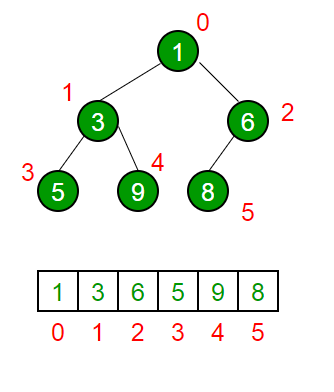
\includegraphics[width=0.5\textwidth]{binaryheap.png}
		\caption{Représentation en mémoire d'un tas binairei - Source: geeksforgeeks.org}
		\label{vs_3}
\end{figure}

Pour chaque noeud (indicé i), nous pouvons obtenir son parent et ses enfants
de la manière suivante:\\
\begin{itemize}
	\item parent(i)  = $\lfloor \frac{i}{2}  \rfloor$
	\item gauche(i) = $i \times 2 + 1$
	\item droite(i) = $i \times 2 + 2 $\\ 
\end{itemize}

Le tas binaire doit supporter les opérations suivantes, dont nos implémentations proviennent de 
\textit{Introduction à l'algorithmique}:
\begin{itemize}
	\item minHeapify(t, i) : cette méthode va rétablir les propriétés du sous tas t à l'indice i
	\item insert(x) : cette méthode va insérer un élément dans notre tas via minHeapify
	\item buildMinHeap(tab) : cette méthode va construire un tas à partir d'un tableau non trié\\
\end{itemize}

Vous pourrez trouver un implémentation d'un tas maximum dans le fichier \textit{heap.c} et 
les tests via le fichier \textit{test\_heap.c}.

\subsection{Implémentation pour notre problème}

Afin de pouvoir utiliser un tas binaire comme file de priorité il va falloir y apporter quelques
modifications liées à notre problème.\\

Nous allons utiliser deux tableaux, elements qui contient les sommets de notre graphe
et keys qui contient les valeurs utilisées pour le tri dans le tas. Dans keys nous
stockerons le coût d'un plus court chemin vers notre sommet plus son heuristique.\\

Un troisième tableau à $n$ éléments sera utilisé afin de savoir si un sommet est
déjà présent et si il y est où se trouve-t-il, si il est absent nous utiliserons la valeur -1.
Nous avons alors indice[i] = argument de i dans \textit{elements}.\\
Ce tableau nous permettra de savoir si un sommet est dans le tas binaire en temps constant,
ce qui nous sera utile pour savoir si nous allons devoir insérer un sommet ou juste 
mettre sa clef à jour. Nous pourrions toujours réinsérer un sommet peut importe qu'il y soit ou
non mais cela nous forcerait a utiliser un tas de taille maximale dynamique, et aurait aussi
pour conséquence de ralentir l'ajout d'éléments dans la file de priorité car le tas 
contiendrait plus d'éléments.\\

Nous aurons aussi besoin des nouvelles fonctions suivantes:
\begin{itemize}
	\item minInsert(elt, key): il s'agit d'une variante de \textit{insert} qui insère un 
		élément et sa clef associée dans notre file de priorité
	\item getMin(t) : cette fonction retourne l'élément minimum dans la file de priorité (l'élément
		à l'indice 0)
	\item extractMin(t): cette fonction va enlever l'élément minimal de la file de priorité
			et le retourner.
	\item decreaseKey(elt, key): cette fonction va baisser la valeur de la clef de l'élément \textit{elt}
			pour y mettre la valeur \textit{key}. Elle s'effectue en temps constant grâce à notre 
			tableau \textit{indices}\\
\end{itemize}

Nous allons alors modifier notre algorithme pour utiliser cette file de priorité afin d'obtenir
plus rapidement l'élément minimum:

\clearpage

\begin{algorithm}
\caption{Algorithme A* avec file de priorité}\label{astar_pq}
\begin{algorithmic}[1]
\Procedure{A*}{$E, \Gamma, l, d \in E, a \in E$}
	\State S = \{d\}, $\pi(d)$ = 0, k = 1, $x_1$ = d, file = $\emptyset$
	\ForAll{$x \in E$\textbackslash$ \{d\}$}
		\State $\pi(x) = \infty$
	\EndFor
	\While{$k < n$ et $\pi(x_k) < \infty$ }
		\ForAll{$y \in \Gamma(x_k) $ tel que $y \not\in S$}
			\State $\pi(y) = $ min[$\pi(y), \pi(x_k) + l(x_k, y)$]
			\If{$y \in file$}
				\State \textsc{decreaseKey}(file, y, pi[y]);
			\Else
				\State \textsc{minInsert}(file, y, pi[y]);
			\EndIf
		\EndFor
		\State x = \textsc{extractMin}(file)  
		\State k = k + 1, $x_k = x$, S = S $\bigcup \{x_k\}$
		\If{$x_k = a$}
			\State \textbf{break}
		\EndIf
	\EndWhile
	
	\State \textbf{return} $\pi$, S
\EndProcedure 

\end{algorithmic}
\end{algorithm}

En comparant à précédemment nous avons désormais \textsc{decreaseKey} qui est en $O(1)$
\textsc{minInsert} qui est en $O(log(n))$ et \textsc{extractMin} en $O(1)$.\\
Nous avions avant un calcul de minimum en $O(n)$.\\
Malgré l'ajout d'une opération en temps logarithmique, nous devrions voir de grandes 
améliorations de temps d'éxécution car nous avons transformé une opération en temps linéaire en
temps constant.

\subsection{Résultats}


\subsection{Autre structures de données possibles}


\end{document}
